\documentclass[10pt]{article}
\usepackage[utf8]{inputenc}
\usepackage[italian]{babel}
\usepackage{multicol}
\usepackage[bookmarks]{hyperref}
\usepackage[a4paper, total={18cm, 25cm}]{geometry}
\usepackage{listings}
\usepackage{graphicx}
\usepackage{makecell}
\graphicspath{ {./img/} }
\usepackage{color}
\definecolor{mygray}{rgb}{0.5,0.5,0.5}
\usepackage{listings}
\usepackage{qtree}
\lstset{
	language=SQL,
	breaklines=true,
	keywordstyle=\bfseries,
	identifierstyle=\ttfamily,
	commentstyle=\color{mygray},
	morekeywords={database, REFERENCES, SCHEMA, AUTHORIZATION, PROCEDURE, WITH, CHECK, OPTION, FOR, EACH, ROW, DECLARE, BEFORE, AFTER, IF, TO, PRIVILEDGES, COMMIT, WORK, ROLLBACK, SORT},
}

\begin{document}
\renewcommand*\contentsname{Indice}
\title{Corso di Basi di Dati A.A. 2020/21\\Progetto "Gestione Progetti ANSA"}
\author{Federico Matteoni\\Mat. 530257}
\date{29/01/2021}
\maketitle
\pagebreak
\section{Descrizione del dominio}
Si vuole progettare un sistema di distribuzione di notizie agli utenti.\\\\
Ogni notizia ha un titolo, autore, testo, data, ora e un'insieme di uno o più argomenti.\\\\
Ogni argomento ha un nome e può essere di tipo Premium o Economy.\\\\
Un utente può essere un autore e poter inviare articoli, firmandoli con proprio nome e cognome.\\\\
Ogni utente può essere Premium o Economy e iscriversi agli argomenti per cui ricevere notizie.\\Un utente Premium può iscriversi ad ogni argomento, mentre un utente Economy può iscriversi solo agli argomenti Economy.\\\\
Un utente Premium può ricevere offerte/sconti speciali.\\\\
Alcuni utenti hanno delle autorizzazioni speciali.
\section{Schema Concettuale}
\begin{center}
	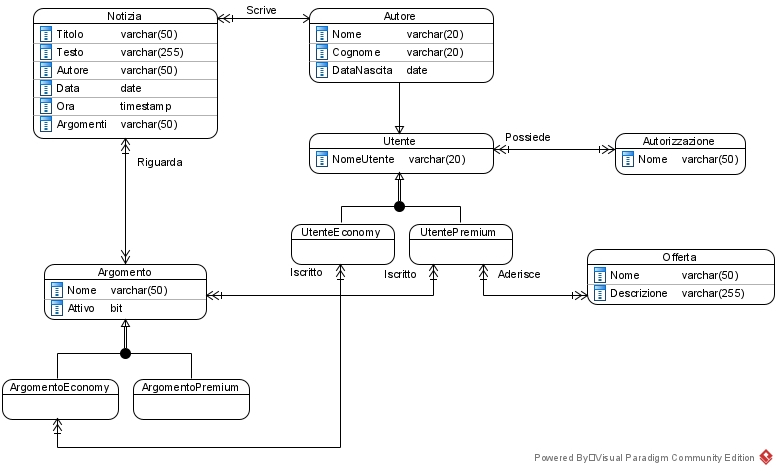
\includegraphics[scale=0.75]{Concettuale.jpg}
\end{center}
\section{Schema Logico Relazionale}
\begin{center}
	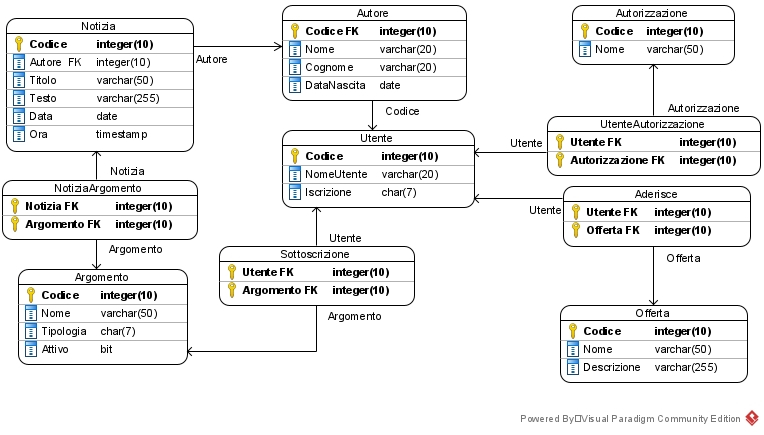
\includegraphics[scale=0.75]{LogicoRelazionale.jpg}
\end{center}
\begin{list}{}{\textbf{Notazione testuale}}
	\item Notizia(\underline{Codice}, Autore*, Titolo, Testo, Data, Ora)
	\item NotiziaArgomento(\underline{Notizia*}, \underline{Argomento*})
	\item Argomento(\underline{Codice}, Nome, Tipologia, Attivo)
	\item Utente(\underline{Codice}, NomeUtente, Iscrizione)
	\item Autore(\underline{Codice*}, Nome, Cognome, DataNascita)
	\item Sottoscrizione(\underline{Utente*}, \underline{Argomento*})
	\item Autorizzazione(\underline{Codice}, Nome)
	\item UtenteAutorizzazione(\underline{Utente*}, \underline{Autorizzazione*})
	\item Offerta(\underline{Codice}, Nome, Descrizione)
	\item Aderisce(\underline{Utente*}, \underline{Offerta*})
\end{list}
\paragraph{Vincoli non catturati graficamente}
\begin{list}{}{}
	\item Ogni utente riferito dalla tabella Aderisce ha il campo "Iscrizione" con valore pari a "premium"
	\item Ogni Argomento con campo "Tipologia" con valore "premium" può essere legato solamente ad un Utente con campo "Tipologia" con valore "premium".
\end{list}
\pagebreak
\section{Query SQL}
\begin{enumerate}
	\item Uso di proiezione, join e restrizione\\
	La lista dei titoli di tutte le notizie di cronaca.
	\begin{lstlisting}
	SELECT Notizia.Titolo
	FROM Notizia
	JOIN NotiziaArgomento ON Notizia.Codice = NotiziaArgomento.Argomento
	JOIN Argomento ON NotiziaArgomento.Argomento = Argomento.Codice
	WHERE Argomento.Nome = "Cronaca"
	\end{lstlisting}
	\item Uso di group by con having, where e sort\\
	La classifica dei giorni del 2020 con più di 5 notizie.
	\begin{lstlisting}
	SELECT Data, COUNT(*) AS Notizie
	FROM Notizia
	WHERE Data.YEAR = 2020
	GROUP BY Data
	HAVING Notizie > 5
	ORDER BY Notizie
	\end{lstlisting}
	\item Uso di join, group by con having e where\\
	La lista degli autori nati dopo il 2000 con più di 10 notizie pubblicate.
	\begin{lstlisting}
	SELECT Nome, Cognome, COUNT(*) AS Notizie
	FROM Autore
	JOIN Notizia ON Notizia.Autore = Autore.Codice
	WHERE DataNascita.YEAR >= 2000
	GROUP BY Autore.Codice
	HAVING Notizie > 10
	\end{lstlisting}
	\item Uso di select annidata con quantificazione esistenziale\\
	La lista degli utenti premium che hanno aderito ad almeno un'offerta.
	\begin{lstlisting}
	SELECT NomeUtente
	FROM Utente
	WHERE EXISTS
		(SELECT Utente
		FROM Aderisce
		WHERE Utente.Codice = Aderisce.Utente)
	\end{lstlisting}
	\item Uso di select annidata con quantificazione universale\\
	La lista degli autori che hanno pubblicato solo notizie di cronaca.
	\begin{lstlisting}
	SELECT Nome, Cognome
	FROM Autore
	WHERE Autore.Codice NOT IN
		(SELECT Notizia.Autore
		FROM Notizia
		JOIN NotiziaArgomento ON Notizia.Codice = NotiziaArgomento.Argomento
		JOIN Argomento ON NotiziaArgomento.Argomento = Argomento.Codice
		WHERE Argomento.Nome <> "Cronaca")
	\end{lstlisting}
	\item Uso di subquery di confronto quantificato usando una subquery\\
	La lista degli utenti con più di metà delle autorizzazioni possibili.
	\begin{lstlisting}
	SELECT NomeUtente, COUNT(UtenteAutorizzazione.Autorizzazione) AS Autorizzazioni
	FROM Utente
	JOIN UtenteAutorizzazione ON Utente.Codice = UtenteAutorizzazione.Utente
	WHERE (Autorizzazioni*2) > (SELECT COUNT(*) FROM Autorizzazione)
	GROUP BY Utente.Codice
	\end{lstlisting}
\end{enumerate}
\pagebreak
\section{Piani di accesso}
\begin{enumerate}
	\item Scrivere un piano di accesso logico delle query 1, 2 e 3\\Per ragioni di spazio, laddove implicito i nomi delle tabelle sono abbreviati con le iniziali.
	\begin{list}{}{}
		\item[1.]		
\Tree [.$\pi$\\N.Titolo [.$\sigma$\\A.Nome="Cronaca" [.$\bowtie$\\NA.Argomento=A.Codice [.$\bowtie$\\N.Codice=NA.Argomento Notizia NotiziaArgomento ] Argomento ] ] ]\\\\
		\item[2.]		
		\Tree [.$\tau$\\Notizie [.$\pi$\\Data,Notizie [.$\sigma$\\Notizie$>$5 [.$\rho$\\COUNT(*)$\leftarrow$Notizie [.Data$\:\gamma\:$COUNT(*) [.$\sigma$\\Data.YEAR=2020 Notizia ] ] ] ] ] ]\\\\
		\item[3.]		
		\Tree [.$\pi$\\Nome,Cognome,Notizie [.$\sigma$\\Notizie$>$10 [.$\rho$\\COUNT(*)$\leftarrow$Notizie [.A.Codice$\:\gamma\:$COUNT(*) [.$\sigma$\\DataNascita.YEAR$\geq$2000 [.$\bowtie$\\N.Autore=A.Codice Autore Notizia ] ] ] ] ] ]
	\end{list}
	\pagebreak
	\item Scrivere un piano di accesso fisico efficiente per i tre piani di accesso logico al punto 1 che non fanno uso di indici e (opzionale) verificare se la sort prima della group by può essere evitata\\Per ragioni di spazio, laddove implicito i nomi delle tabelle sono abbreviati con le iniziali.\\\\1.\Tree [.Project(N.Titolo) [.NestedLoop(NA.Argomento=A.Codice) [.Filter(A.Nome="Cronaca") TableScan(Argomento) ] [.NestedLoop(N.Codice=NA.Argomento) TableScan(Notizia) TableScan(NotiziaArgomento) ] ] ]\\\\\\
		2.
		\Tree [.Sort(COUNT(*)) [.Project(Data,COUNT(*)) [.Filter(COUNT(*)$>$5) [.GroupBy(Data,COUNT(*)) [.Filter(Data.YEAR=2020) SortScan(Notizia,Data) ] ] ] ] ]\\\\Posso evitare la Sort prima della GroupBy ordinando immediatamente la tabella Notizia in fase di\\scansione.\\\\\\
		3. \Tree [.Project(Nome,Cognome,COUNT(*)) [.Filter(COUNT(*)$>$10) [.GroupBy(A.Codice,COUNT(*)) [.Filter(DataNascita.YEAR$\geq$2000) [.SortMerge(N.Autore=A.Codice) SortScan(Autore,Codice) SortScan(Notizia,Autore) ] ] ] ] ]\\\\Posso evitare la Sort prima della GroupBy ordinando immediatamente la tabella Autore in fase di scansione.
		\pagebreak
	\item Scrivere un piano di accesso fisico efficiente per i tre piani di accesso logico al punto 1 che fanno uso di due indici (o comunque del numero massimo di indici possibili) e (opzionale) verificare se la sort prima della group by può essere evitata\\Per ragioni di spazio, laddove implicito i nomi delle tabelle sono abbreviati con le iniziali.\\\\1.\Tree [.Project(N.Titolo) [.IndexNestedLoop(NA.Argomento=A.Codice) [.Filter(A.Nome="Cronaca") TableScan(Argomento) ] [.IndexFilter(Idx$_{\textsl{NA.Argomento}}$,NA.Argomento=A.Codice) [.IndexNestedLoop(NA.Argomento=N.Codice) TableScan(Notizia) IndexFilter(NotiziaArgomento,\\Idx$_{\textsl{NA.Argomento}}$),\\NA.Argomento=N.Codice ] ] ] ]\\\\\\
		2.
		\Tree [.Sort(COUNT(*)) [.Project(Data,COUNT(*)) [.Filter(COUNT(*)$>$5) [.GroupBy(Data,COUNT(*)) [.Sort(Data) [.IndexFilter(Idx$_{\textsl{Data}}$,Data.YEAR=2020) IndexScan(Notizia,Idx$_{\textsl{Data}}$) ] ] ] ] ] ]\\\\\\
		3. \Tree [.Project(Nome,Cognome,COUNT(*)) [.Filter(COUNT(*)$>$10) [.GroupBy(A.Codice,COUNT(*)) [.Filter(DataNascita.YEAR$\geq$2000) [.IndexNestedLoop(N.Autore=A.Codice) SortScan(Autore,Codice) IndexFilter(Notizia,Idx$_{\textsl{Autore}}$,N.Autore=A.Codice) ] ] ] ] ]\\\\Posso evitare la Sort prima della GroupBy ordinando immediatamente la tabella Autore in fase di scansione.
\end{enumerate}
\end{document}